 \documentclass[12pt]{article}
 
 \usepackage[margin=1in]{geometry} 
 \usepackage{amsmath,amsthm,amssymb}
 \usepackage{pgfplots}
 
 \newcommand{\N}{\mathbb{N}}
 \newcommand{\Z}{\mathbb{Z}}
 
 \newenvironment{theorem}[2][]{\begin{trivlist}
 		\item[{\bfseries #1}\hskip \labelsep {\bfseries #2.}]}{\end{trivlist}}
 \newenvironment{lemma}[2][Lemma]{\begin{trivlist}
 		\item[\hskip \labelsep {\bfseries #1}\hskip \labelsep {\bfseries #2.}]}{\end{trivlist}}
 \newenvironment{exercise}[2][Exercise]{\begin{trivlist}
 		\item[\hskip \labelsep {\bfseries #1}\hskip \labelsep {\bfseries #2.}]}{\end{trivlist}}
 \newenvironment{reflection}[2][Reflection]{\begin{trivlist}
 		\item[\hskip \labelsep {\bfseries #1}\hskip \labelsep {\bfseries #2.}]}{\end{trivlist}}
 \newenvironment{proposition}[2][Proposition]{\begin{trivlist}
 		\item[\hskip \labelsep {\bfseries #1}\hskip \labelsep {\bfseries #2.}]}{\end{trivlist}}
 \newenvironment{corollary}[2][Corollary]{\begin{trivlist}
 		\item[\hskip \labelsep {\bfseries #1}\hskip \labelsep {\bfseries #2.}]}{\end{trivlist}}
 \theoremstyle{remark}
 \newtheorem*{remark}{Remark}
 
 \begin{document}
 	
 	%\renewcommand{\qedsymbol}{\filledbox}
 	
 	\title{Homework 1}
 	\author{David Miller \\ 
 		MAP 5165: Methods in Applied Math I} 
 	
 	\maketitle
 	
 	\subsection*{Problem 1}
 	
 	\textit{(a) State the contraction mapping theorem for R.}
 	
 	\begin{theorem}{Contraction Mapping Theorem}
 		Let $(R,d)$ be a metric space. Then a map 
 		$$ f: R \rightarrow R $$
 		is called a contraction mapping on $R$ if there exists some $c \in [0,1)$ such that 
 		$$ d(f(x), f(x^\prime)) \leq cd(x, x^\prime) $$
 		for all $x, x^\prime$ in $R$.
 	\end{theorem}
 	
 	\vspace{1cm}
 	\noindent \textit{(b) Show that if $f(x)$ is a contraction on $R$, then $g(x)$ = $f(f(x))$ is also a contraction on $R$.}
 	
 	\begin{proof}
 		Since $f$ is a contraction, we get that 
 		$$ f:X \rightarrow X_R, $$
 		where $X_R$ is a restricted domain $X_R \subsetneq X$. Then 
 		$$ g = f \circ f = f:X_R \rightarrow Y. $$
 		Since $f$ is a contraction we get that $Y = X_{RR}$ is a restricted domain $X_{RR} \subsetneq X_R \subsetneq X$. Therefore $g$ maps $X$ to some restricted subset of $X$ showing that it is a contraction.
 	\end{proof}
 	\begin{remark}{1}
 		Essentially a contraction mapping $f: X \rightarrow X$ maps points closer together. For all $x \in X$ we have that all points $y$ in $B_r(x)$ are mapped to $B_q(x)$ for $q < r$ and $r > 0$. It's also important to note that if $f:\mathbb{R} \rightarrow \mathbb{R}$ we ca rewrite the theorem as 
 		$$ \frac{d(f(x), f(x^\prime))}{d(x, x^\prime)} = \frac{\vert f(x^\prime) - f(x) \vert}{\vert x^\prime - x \prime \vert} = \Big\vert \frac{f(x^\prime) - f(x)}{x^\prime - x} \Big\vert \leq c \quad \text{for some } c \in [0.1).$$
 		What this means is for any function $f$ that maps $\mathbb{R}$ to $\mathbb{R}$ the derivative's magnitude at each point $x$ must be less than 1 for it to be a contraction mapping. This can be shown by
 		$$ \lim\limits_{x \rightarrow x^\prime} \frac{d(f(x), f(x^\prime))}{d(x, x^\prime)} = \Big\vert \lim\limits_{x \rightarrow x^\prime} \frac{f(x^\prime) - f(x)}{x^\prime - x}  \Big\vert = \vert f^\prime(x^\prime) \vert \leq c $$
 		for all $x^\prime \in \mathbb{R}$.
 	\end{remark}
 	
 	\vspace{1cm}
 	\noindent \textit{(c) Which of the following are contraction maps? Explain your answer.} 
 	\begin{proposition}{1}
 		A line $f(x) = mx +b$ such that $\vert m \vert \geq 1$ is not a contraction mapping.
 	\end{proposition}
 	\begin{proof}
 		The distance between two points $f(x)$ and $f(x^{\prime})$ on a line is $\vert f(x) - f(x^\prime) \vert = \vert (mx + b) - (mx^\prime + b) \vert = \vert m(x - x^\prime) \vert = \vert m \vert \vert x - x^\prime \vert$. It's easy to see that for this to be a contraction mapping $\vert m \vert < 1$.
 	\end{proof}
 	\noindent \textit{(c1) f(x) = 3x - 4} \\ \\
 	Not a contraction mapping. See Proposition 1. \\ \\
 	\noindent \textit{(c2) f(x) = -$\frac{x}{2}$ + 10} \\ \\
 	Is a contraction mapping on $\mathbb{R}$. See Proposition 1. \\ \\
 	\noindent \textit{(c3) f(x) = $\frac{1}{3}$ - x} \\ \\
 	Not a contraction mapping. See Proposition 1. \\ \\
 	\noindent \textit{(c4) f(x) = cos(x)} \\ \\
 	Is a contraction mapping on the interval $[-\frac{\pi}{2} + \epsilon, \frac{\pi}{2} - \epsilon]$ for any $0 < \epsilon \leq \frac{\pi}{2}$.
 	\begin{proof}
 		Let's parametrize the circle clockwise with $x = 0$ at the point $(cos(0), sin(0)) = (1,0)$.
 		
 		\begin{center}
 			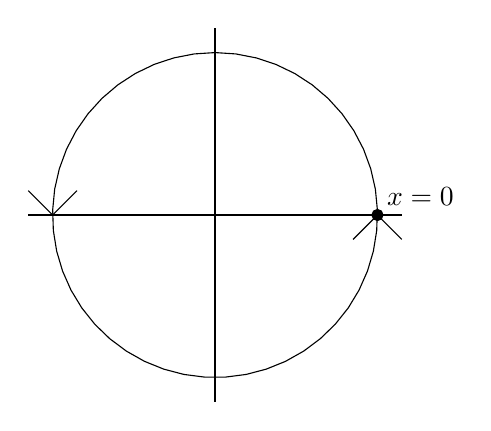
\begin{tikzpicture}
 			\begin{axis}[
 			trig format plots=rad,
 			axis equal,
 			hide axis
 			]
 			
 			\node at (axis cs:1,0) [anchor=south west] {$x = 0$};
 			\addplot [only marks] table {
 				1 0
 			};
 			\addplot [domain=0:2*pi, samples=50, black] ({sin(x)}, {cos(x)});
 			\addplot [domain = 0:0.15, samples = 50, black] ({x-1}, {x});
 			\addplot [domain = 0:0.15, samples = 50, black] ({x-1.15}, {-x+0.15});
 			\addplot [domain = 0:0.15, samples = 50, black] ({x+1}, {-x});
 			\addplot [domain = 0:0.15, samples = 50, black] ({x+0.85}, {x-0.15});
 			\addplot [domain = -1.15:1.15, samples=50, black] ({x}, {0});
 			\addplot [domain = -1.15:1.15, samples=50, black] ({0}, {x});
 			\end{axis}
 			\end{tikzpicture}
 		\end{center}
 		The traversal of the function
 		$$ f: \mathbb{R} \rightarrow [-1,1] $$
 		$$ f(x) = cos(x) $$
 		can be thought of as the following: as we travel along the curve we travel in domain space and as we travel along the horizontal axis we travel in codomain space. We can do this because the curve $(rcos(x), rsin(x)) = (cos(x), sin(x)) = (f(x), sin(x))$ is parametrized w.r.t. x. Now we pick two random points $x$ and $x^\prime$, then we can see that $d(x,x^\prime)$ is an arc on the circle while $d(f(x), f(x^\prime))$ is a line segment 
 		\begin{center}
 			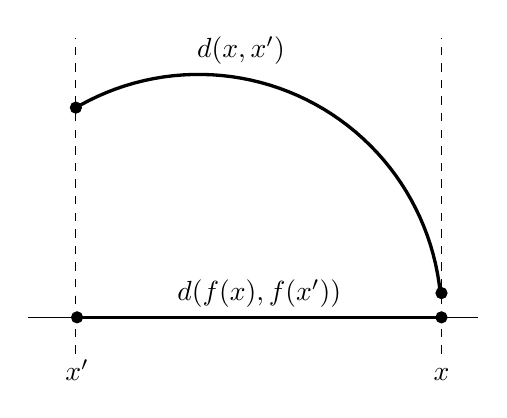
\begin{tikzpicture}
 			\begin{axis}[
 			trig format plots=rad,
 			axis equal,
 			hide axis
 			]
 			\node at (axis cs:1,-0.3) [anchor=south] {$x $};
 			\node at (axis cs:-0.5,-0.3) [anchor=south] {$x ^\prime$};
 			\node at (axis cs:0.175,1) [anchor=south] {$d(x,x^\prime)$};
 			\node at (axis cs:0.25,0.0) [anchor=south] {$d(f(x),f(x^\prime))$};
 			\addplot [only marks] table {
 				1 0
 				-0.50485 0.863209
 				1 .09983342
 				-0.5 0
 			};
 			\addplot [domain = -.15:1.15, samples=50, black, dashed] ({-0.505}, {x});
 			\addplot [domain = -0.15:1.15, samples=50, black, dashed] ({1}, {x});
 			\addplot [domain = -0.701:1.15, samples=50, black] ({x},{0});
 			\addplot [domain = -0.5:1, samples=50, black, very thick]({x},{0});
 			\addplot [domain = -0.25:1.73, samples=50, black, very thick] ({cos(x+.35)},{sin(x+.35)});
 			\end{axis}
 			\end{tikzpicture}
 		\end{center}
 		Since $d(f(x),f(x^\prime))$ is always a straight line and $d(x,x^\prime)$ is never a straight line, we have that $d(f(x),f(x^\prime)) < d(x,x^\prime)$. Therefore the distance traveled in the domain is always greater than the distance traveled in the range. However since $f(x) = cos(x)$ is a mapping from $\mathbb{R} \rightarrow \mathbb{R}$ we know from remark 1 that it is only a contraction mapping whenever $\vert f^\prime(x) \vert < 1$. Since $f^\prime(x) = sin(x)$ and $\vert f^\prime(\frac{\pi}{2} + n\pi) \vert = 1$ it follows that $cos(x)$ is a contraction mapping on any interval of the form $[-\frac{\pi}{2} + \epsilon, \frac{\pi}{2} - \epsilon]$ for any $0 < \epsilon \leq \frac{\pi}{2}$.
 	\end{proof}
 	\noindent \textit{(c5) f(x) = $\frac{1}{2}$sin(x)} \\ \\
 	Is a contraction mapping on $\mathbb{R}$.
 	\begin{proof}
 		This proof is of a similar flavor as part $(c4)$. This time let the travel in range space take part in the vertical axis. Then it is easy to see that showing the vertical line segment is strictly less than the arc length. However in this case we have that $ \vert f^\prime(x) \vert = \vert \frac{1}{2}cos(x) \vert$ and this value is never greater than 1. It then follows that $f(x)$ is a contraction mapping on all of $\mathbb{R}$.
 	\end{proof}
 	
 	\newpage 
 	
 	\noindent \textit{(c6) f(x) = exp(-$x^2$)} \\ \\
 	Is a contraction mapping on $\mathbb{R}$.
 	\begin{proof}
 		\begin{align*}
 		& \vert e^{-x^2} - e^{-y^2} \vert \leq c \vert x - y \vert \\
 		& \frac{\vert e^{-x^2} - e^{-y^2} \vert}{\vert x - y \vert} = \Big\vert \frac{e^{-x^2} - e^{-y^2}}{x - y} \Big\vert \leq c \\
 		& \lim\limits_{\Delta x \rightarrow 0} \Big\vert \frac{e^{-x^2} - e^{-(x+\Delta x)^2}}{x - (x + \Delta x)} \Big\vert \leq \lim\limits_{\Delta x \rightarrow 0} c \\
 		& \lim\limits_{\Delta x \rightarrow 0} \vert -2(x + \Delta x)e^{-(x+\Delta x)^2} \vert \leq c \quad (\text{L'Hoptial's Rule}) \\
 		& \vert -2xe^{-x^2} \vert \leq c \Rightarrow \vert \frac{2x}{e^{x^2}} \vert \leq c 
 		\end{align*}
 		Since $e^{-x^2} > 2x$ for all $x$ we have that $\frac{2x}{e^{x^2}} < 1$ for all $x$ and therefore $c < 1$.
 	\end{proof}
 	
 	\newpage
 	
 	\subsection*{Problem 2}
 	
 	\textit{Consider the initial value problem}
 	$$ \dot{x} = \vert x \vert^{\alpha/\beta}, \quad x(0) = 0, $$
 	\textit{where $\alpha$ and $\beta$ are positive integers with no common factors.} \\ \\
 	\textit{(a) Show that there exists an infinite number of solutions if $\alpha < \beta$.} \\ \\
 	When $x > 0$ we have that 
 	\begin{align*}
 	& \dot{x} = f(x) = x^{\frac{\alpha}{\beta}} \\
 	\Rightarrow & f^\prime(x) = \frac{\alpha}{\beta}x^{\frac{\alpha}{\beta} - 1} 
 	\end{align*}
 	and when $x < 0$ we have that
 	\begin{align*}
 	& \dot{x} = f(x) = -x^{\frac{\alpha}{\beta}} \\
 	\Rightarrow & f^\prime (x) = -\frac{\alpha}{\beta}x^{\frac{\alpha}{\beta} - 1}.
 	\end{align*}
 	From this we can conclude that 
 	\begin{align*}
 	f^\prime(x) & = \frac{\alpha}{\beta}sign(x)x^{\frac{\alpha}{\beta} - 1} \\
 	& = \frac{\alpha}{\beta}\frac{sign(x)}{x^{1-\frac{\alpha}{\beta}}} \\
 	& = \frac{\alpha}{\beta}\frac{sign(x)x^{\frac{\alpha}{\beta}}}{x}
 	\end{align*}
 	Rewriting the Lipschitz inequality we have
 	\begin{align*}
 	& \frac{\vert f(y) - f(x) \vert}{\vert y - x \vert} \leq c \quad \text{for some } c > 0
 	\end{align*}
 	If we let $x = 0$ and $y \rightarrow 0^+$ we have
 	\begin{align*}
 	\lim\limits_{y \rightarrow 0^+} \frac{\vert f(y) - f(0) \vert}{ \vert y - 0 \vert} =\frac{f(y) - f(0)}{y - 0} = f^\prime(0) = \infty. 
 	\end{align*}
 	This shows that the closer you get towards 0 there is no $c$ you can choose that will satisfy the Lipschitz inequality. Therefore our IVP is not Lipschitz continuous around $(0, x(0)) = (0,0)$ and therefore has infinitely many solutions. \\ \\
 	
 	\newpage 
 	
 	\noindent \textit{(b) Show that there is a unique solution if $\alpha > \beta$.} \\
 	\begin{proof}
 		When $\alpha > \beta$ we have that 
 		\begin{align*}
 		& \dot{x} = f(x) = x^{\frac{\alpha}{\beta}} \\
 		& f^\prime(x) = -\frac{\alpha}{\beta}x^{\frac{\alpha}{\beta}-1} \quad x< 0 \\
 		& f^\prime(x) = \frac{\alpha}{\beta}x^{\frac{\alpha}{\beta}-1} \quad x< 0 \\
 		& f^\prime(x) = 0 \quad x = 0 \\
 		\Rightarrow & f^\prime(x) = \frac{\alpha}{\beta}sign(x)x^{\frac{\alpha}{\beta}-1}
 		\end{align*}
 		It's easy to see that $f^\prime(x)$ is continuous. From Picard's Theorem we have that our IVP has a unique solution.
 	\end{proof}
 	
 	\newpage
 	
 	\subsection*{Problem 3}
 	
 	\textit{Consider the dynamical system}
 	$$ \dot{x} = x^\alpha, \quad x(0) = x_0 > 0. $$
 	\textit{Show that if $\alpha > 1$ there exists a finite time $t_* = t_*(\alpha, x_0) < \infty$ such that}
 	$$ \lim\limits_{t \rightarrow t_*^-} x(t) = \infty $$
 	\begin{proof} For this proof we will use Picard's Theorem:
 		\begin{theorem}{Picard's Theorem}
 			Consider the initial value problem
 			$$ y^\prime = f(x,y), \quad y(x_0) = y_0. $$
 			Suppose $f(x,y)$ and $\frac{\partial f}{\partial x}$ are continuous functions in some open rectangle $R = \{(x,y): a < x < b, c < y < d\}$ that contains the point $(x_0, y_0)$. Then the IVP has a unique solution in some closed interval $I = [x_0 - h, x_0 + h]$ where $h > 0$.
 		\end{theorem}    
 		Since $\dot{x} = x^\alpha$ is continuous we have that $x(t)$ has a unique solution. This is important to note because unique solution implies only having to find one $t_*$ rather than infinitely many. Solving the IVP
 		\begin{align*}
 		& \dot{x} = \frac{dx}{dt} = x^\alpha \\
 		\Rightarrow & \int x^{-\alpha} dx = \int dt \\
 		& \frac{x^{\alpha+1}}{-\alpha + 1} = t + c \\
 		& x(t) = \bigg[(-\alpha + 1)t + c\bigg]^{\frac{1}{-\alpha + 1}} \\
 		& x(0) = x_0 = c^{\frac{1}{-\alpha + 1}} \\
 		\Rightarrow & c = x_0^{-\alpha + 1} \\
 		& x(t) = \bigg[(-\alpha + 1)t + x_0^{-\alpha + 1}\bigg]^{\frac{1}{-\alpha + 1}}
 		\end{align*} 
 		Since $\alpha > 1$ we can rewrite $x(t)$ as
 		$$ x(t) = \bigg[\frac{1}{(-\alpha + 1)t + x_0^{-\alpha + 1}}\bigg]^{\alpha - 1} $$
 		The function $x(t)$ will blow up to infinity when the numerator is zero.
 		\begin{align*}
 		& (-\alpha + 1)t_* + x_0^{-\alpha + 1} = 0 \\
 		& t_* = -\frac{x_0^{-\alpha + 1}}{-\alpha + 1} = \frac{x_0^{-\alpha + 1}}{\alpha - 1}
 		\end{align*}
 		Its easy to verify that $t_* > 0$ and from this we can see as time progresses the IVP will blow up. This proves that 
 		\begin{align*}
 		& \lim\limits_{t \rightarrow t_*^-} x(t) = \infty \quad \text{for } t_* = \frac{x_0^{-\alpha + 1}}{\alpha - 1} > 0
 		\end{align*}
 	\end{proof}
 	
 	\newpage
 	
 	\subsection*{Problem 4}
 	
 	\textit{Find the first three successive approximations $x_1(t), x_2(t),$ and $x_3(t)$ for the initial value problem}
 	$$ \dot{x} = x^2, \quad x(0) = 1. $$
 	The solution to the IVP problem is the associated integral equation
 	\begin{align*}
 	x(t) = x(0) + \int\limits_{t_0}^{t} f(s, x(s)) ds
 	\end{align*}
 	where $f(t,x) = x^2$. Using the Picard iteration 
 	\begin{align*}
 	x_n(t) = x_{0} + \int\limits_{t_0}^{t} f(s, x_{n-1}(s)) ds
 	\end{align*}
 	and $x(0) = x_0 = 1$, $t_0 = 0$ we get
 	\begin{align*}
 	x_1 & = 1 + \int\limits_{t_0}^t (1)^2 ds = 1 + t \\
 	x_2 & = 1 + \int\limits_{t_0}^t (1+s)^2 ds = 1 + \Big(t + t^2 + \frac{1}{3}t^2\Big)\Big|_{0}^t = 1 + t + t^2 + \frac{1}{3}t^3 \\
 	x_3 & = 1 + \int\limits_{t_0}^t (1 + t + t^2 + \frac{1}{3}t^3)^2 ds \\
 	& = \int\limits_{t_0}^t (1 + 2s + 3s^2 + \frac{8}{3}t^3 + \frac{5}3)t^4 + \frac{2}{3}t^5 + \frac{1}{9}t^6 ds \\
 	& = \Big(1 + s + s^2 + s^3 + \frac{2}{3}s^4 + \frac{1}{3}s^5 + \frac{1}{9}s^5 + \frac{1}{63}s^7\Big)\Big|_0^t \\
 	& = 1 + t + t^2 + t^3 + \frac{2}{3}t^4 + \frac{1}{3}t^5 + \frac{1}{9}t^5 + \frac{1}{63}t^7
 	\end{align*}
 	It is clear to see that if we continue the iteration we will get that 
 	\begin{align*}
 	x_n = \sum\limits_{i=0}^n t^i + \mathcal{O}(t^{n+1}) 
 	\end{align*}
 	Since the Taylor Series expansion for $\frac{1}{1-t}$ is $\sum_{n=0}^\infty t^n$ we see that $x_n \rightarrow \frac{1}{1-t}$ as $n \rightarrow \infty$.
 	
 \end{document}